\begin{center}
	{\bf\Large 格式说明}
\end{center}

\bigskip\bigskip

为了突出重点内容,区分不同要求,本讲义通过使用不同字体、色彩、背景
和文本框对内容加以区分,说明如下:

\bigskip\bigskip

宋体字:正文;

\bigskip\bigskip

{\kaishu 楷体字:}专有名词或概念;

\bigskip\bigskip

{\bf 黑体字}:重要概念或结论,各类标题;

\bigskip\bigskip

{\b 蓝色字体}:重要的附注或说明;

\bigskip\bigskip

{\color{red} 红色字体:}重要说明,务必重视;

\bigskip\bigskip

\begin{thx}
	深蓝色边框,白色底色文本框:重要概念或结论;
\end{thx}

\bigskip\bigskip

\begin{ext}
	深绿色边框,绿色底色文本框:课后作业或练习题;
\end{ext}

\bigskip\bigskip

\begin{shaded}
	黑色背景文本框:扩展阅读知识,了解即可,不要求掌握;
\end{shaded}

\bigskip\bigskip

边栏文本:\ps{附注和说明。}

\newpage

\section{课程简介}

\subsection{学什么}

高等数学是大学工科专业必修的数学基础课,通常和{\it 线性代数}、{\it 概率论与数理统计}统称
为{\it 工程数学}。

我们所说的高等数学,在国外一般就叫做{\it 微积分},而且通常分为{\it 一元函数微积分}
和{\it 多元(高维)微积分}两个部分。而国外所说的{\it 高等数学}就是我们说的工程数学。

我们一般认为,微积分诞生于17世纪中叶,当时的两位数学巨匠Newton(1642-1726)和
Leibniz(1646-1716)分别独立
创立了微积分的理论,并最终被视为微积分的共同创始人。但是,我们必须认识到的是,
一门系统、复杂的理论,不可能仅仅是极个别人的创造。正如Newton的名言,“{\it If 
I have seen further, it is by standing on the shoulders of
giants.}”,在两位大师生前和生后,众多杰出的数学家都为微积分理论的发展作出了
贡献,其中既包括Fermat(1607-1665)、Barrow(1630-1677)、
Descartes(1596-1650)%、Huygens(1629-1695)、Wallis(1616-1703)
等人的奠基性工作,也包括Cauchy(1789-1857)、D.Bernoulli(1700-1782)、
Lagrange(1736-1913)、Weierstrass(1815-1897)、Cantor(1845-1918)、
Taylor(1685-1731)、Euler(1707-1783)、d'Alembert(1717-1783)
%、Laplace(1749-1827)、Agnesi(1718-1799)
使之严谨化以和完善,更包括Dirichlet(1805-1859)、Riemann(1826-1866)、
Lebesgue(1875-1941)、Fourier(1772-1837)以及后世很多数学家在{\it 分析
学}上的深入探索。今天我们所学习的微积分,虽然只是这一学科
\ps{更准确的说法应该叫分析学,它和几何学、代数学并称现代数学的三大分支,
三者各自拥有庞大的理论体系,在它们的交汇处诞生了众多重要而又生机勃勃的
数学前沿分支}的基础部分,但要说其中融汇了300多年来众多近现代数学家
的杰出成就,是绝对实至名归的。

% \begin{figure}[htbp]
% 	\centering\scalebox{0.3}{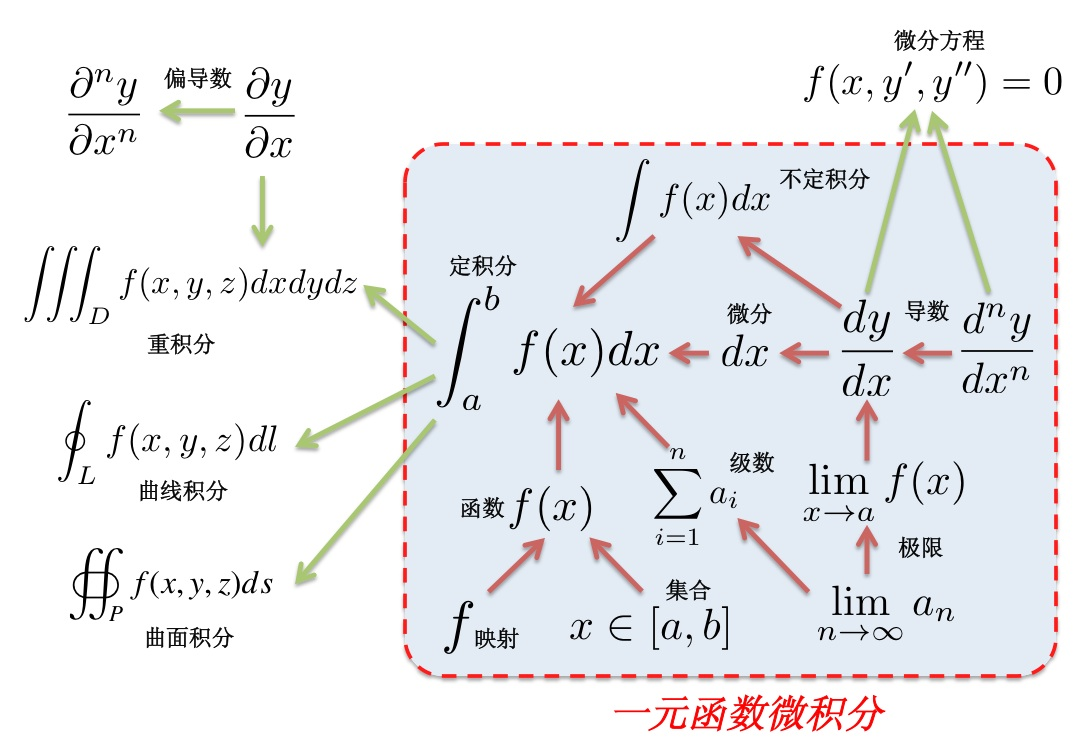
\includegraphics{./images/ch1/AM_architecture.jpg}}
% 	\caption{微积分中的主要概念及其关系\;
% 	({\it 个人整理,仅供参考})}
% % 	\label{图:0.1}
% \end{figure}

% \begin{center}
% 	\scalebox{0.3}{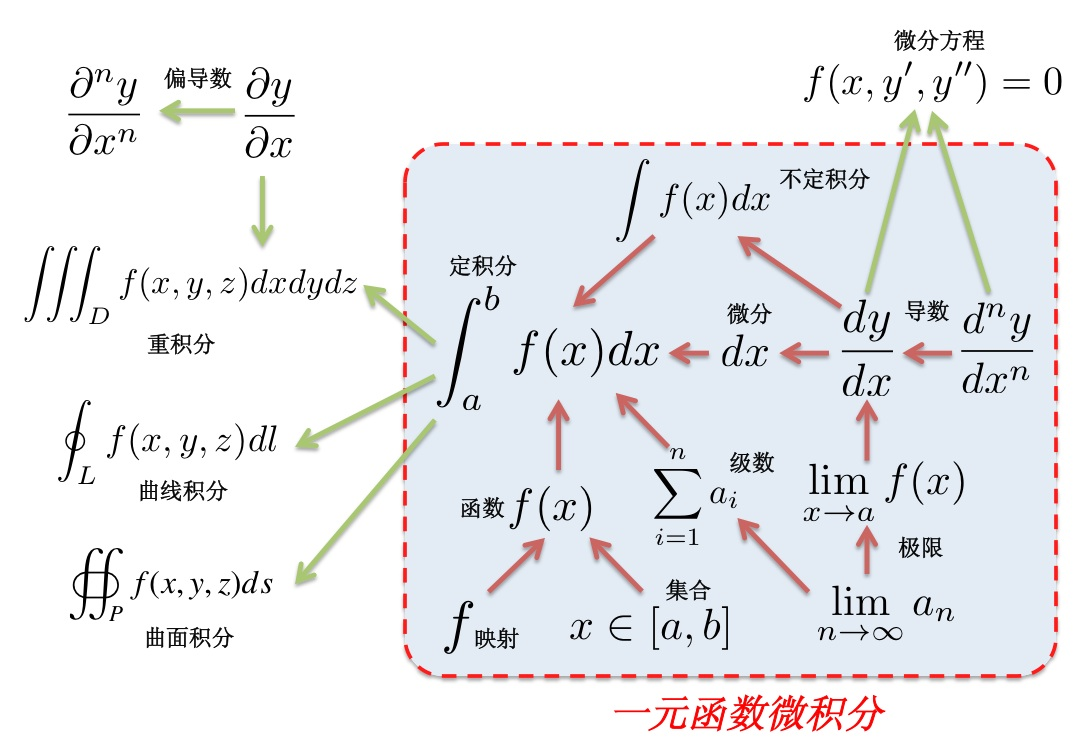
\includegraphics{./images/ch1/AM_architecture.jpg}}
% % 	\ps{上课前画好}
% \end{center}

\begin{center}
	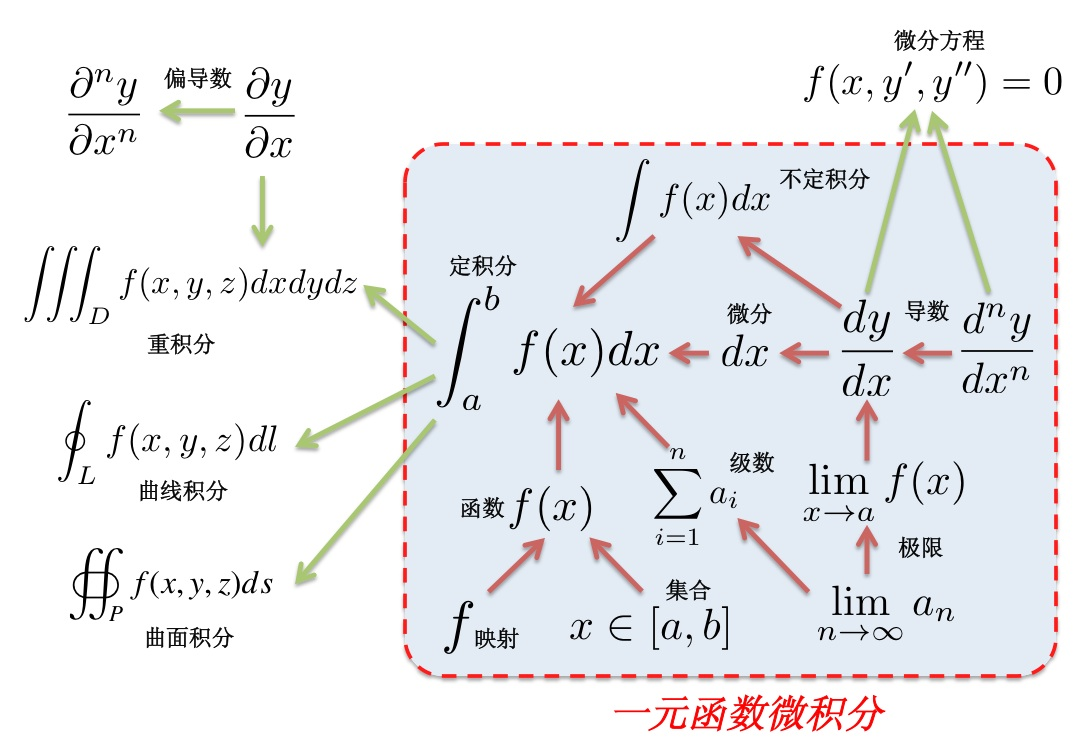
\includegraphics[width=0.8\textwidth]{./images/ch1/AM_architecture.jpg}
	
	{微积分中的主要概念及其关系\;
	({\it 个人整理,仅供参考})}
\end{center}

\begin{itemize}
	  \item {\bf Wikipedia——微积分(Calculus)} 
	\begin{itemize}
	  \item Latin: {\it a small stone used for counting}  
	  \item {\it a branch of mathematics focused on \underline{limits, functions,
	  	derivatives, integrals, and infinite series}} 
  	  \item {\it widespread application in \underline{science, economics,} 
  	  and \underline{engineering}} 
	  \item {\it constitues a major part of modern mathematics}
	  \item {\it 微}的意思是很小的东西,如微生物,{\it 积}就是加起来的意思,
	  {\it 积分}的意思就是把极小的东西加起来。微,是积的相反。 
	\end{itemize}
	\item {\bf John von Neumann} ({\small\it The Mathematician, 1947})
	\begin{itemize}
	  \item {\it The calculus was the \underline{first achievement} of modern
	  mathematics, and it is difficult to overestimate its importance.}
	\end{itemize} 
\end{itemize}

\subsection{为什么学}

微积分为什么如此重要,毫无疑问,与其在众多领域的应用密不可分,甚至可以说,
在其中绝大多数的问题中,微积分的作用是无可替代的。任何一门工科类的专业课程,
只要涉及与连续运动(变化)相关的问题,都不可避免地会以微积分作为其预备知识,
或者说,将这些课程视为微积分的应用也不为过。

当然,微积分不总是“美丽”的,因为它的美可能不是那么显而易见。我们很难用一两句话
来描述,微积分到底有什么用?它美在哪里?但是,一旦你理解了微积分背后的深刻思想,
开始能够将其应用于解决一些实际问题,或者通过它理解一些最前沿的科技成就时,
你一定会对它的美产生深深地赞叹,也许那时,再回头来看微积分的重要性也就不言而喻了。

学习微积分的过程也许会有些枯燥甚至痛苦\ps{“从前有棵树,叫高数,上面挂了很多人”}
,但它无疑是值得的,能够从看似单调痛苦的过程中领略数学的美丽,发现它的深刻与强大,
也是它作为“{\it 大学第一课}”\ps{无论从体量、难度还是学习的先后来看}所期望带给
大家的体验。

\begin{shaded}
	{\bf 知乎:学数学有什么好处?我们为什么要学数学?}
	\begin{itemize}
	  \item Engles:{\it 数学是一门研究现实世界的数量关系和空间形式的科学。}数学具有:
	  抽象性、精确性和应用的广泛性
	  \item Marx:{\it 一种科学只有在成功运用数学时,才算达到了真正完善的地步。}
	  \item Galileo:{\it “数学符号就是上帝用来书写自然这一伟大著作的统一语言,
	  不了解这些文字就不可能懂得自然的统一语言,只有用数学概念和公式所表达的物理世界
	  的性质才可认识……”}
	  \item Gauss:{数学是科学的女王}
	  \item 韩寒:{\it
	  我们生活中用到的数学估计到小学三年级就已经够用了。}然而在之后我们多年来学习的数学,
	  实际上塑造了我们一种理性的、条理的、系统化的思维方式。这种思维方式在我们解决自己
	  一生中遇到的诸多问题时,都有非常重要的作用。比如慎密的思考、分类的思想、排序的思想等。
	  很多东西其实都带有学习数学这个过程产生的影响,只是由于其作用方式非常隐晦,
	  也不容易被追溯其源头,我们平时不容易注意到罢了。
	  \item 王小波:{\it 我上大学时,有一次我的数学教授在课堂上讲到:我现在所教的数学,
	  你们也许一声都用不到,但我还要教,因为这些知识是好的,应该让你们知道。”}
	  \item 崔钢:{\it\b 1,用通用简洁的方式来表达自然规律。2,提供一些问题的分析手段。
	  3,提供认识世界的一种模式。4,了解自己的智力水平。.}
	\end{itemize}
	{\bf 豆瓣:为什么没人喜欢学习高等数学?木遥}
	\begin{itemize}
% 	  \item {\it 我完全不能理解,一个非数学或物理专业的学生怎么可能从这样的教育中获得一丝一毫的教益?
% 	  他怎么可能不发自内心地痛恨这门课程,然后在考完试之后的一个小时之内把所有内容忘得精光?
% 	  象三角代换这类积分技巧,不要说一个普通的心理学或者经济学专业的学生一辈子都用不到,
% 	  就连我也一辈子都用不到。就算在极其罕见的情形下需要求解这类问题,也完全可以求助于
% 	  wolframalpha.com 或者类似的工具。
	  \item 在我看来,在二十一世纪还要求一个普通学生手算积分,
	  就像是要求一个汽车驾校学员一定要从骑马学起一样。
	  \item \ldots 一本基于数学家思维方式写出来的教材,亦即在每一个课题上从最基本的定义
	  和定理开始堆砌,直到超出教材所可能涵盖的水平为止
	  \item 如果是我来编写大学数学教材,我会争取让每一个在大学里读过数学课的人都能回答这样的问题:
	  为什么人们能精确预测几十年后的日食,却没法精确预测明天的天气;为什么人们可以通过 https 
	  安全地浏览网页而不会被监听;为什么全球变暖的速度超过一个界限就变得不可逆了;
	  为什么把文本文件压缩成 zip 体积会减少很多,而 mp3 文件压缩成 zip 大小却几乎不变;
	  民生统计指标到底应该采用平均数还是中位数;当人们说两种乐器声音的音高相同而音色不同的时候
	  到底是什么意思\ldots\ldots这不是什么「趣味数学」,这就是数学。基础、重要、深刻、美的数学。
	  \item 在我的设想里,这才是大学基础数学教育所应该达成的任务。
	  {\it 不是培养一个非数学专业的现代人在数学领域的专业素质(这是无论如何也不可能成功的),
	  而是让一个人能够在非专业的前提下最大程度地掌握真正有用的现代数学知识,
	  了解数学家们的工作怎样在各个层面上和社会产生互动,以及社会在这个领域的投资得到了怎样的回报。}
	  别的科学门类的基础教育也应当是这样。
	\end{itemize}
	{\bf 知乎:学习编程及做程序员对微积分的要求高吗?}
\end{shaded}

\begin{itemize}
  \item {\bf 数学的三大功能}
  \begin{enumerate}
    \item 为学习其他知识(课程)提供数学工具
    \item 培养理性思维
    \item 弘扬数学文化
  \end{enumerate}
  \item {\bf 数学素质}
  \begin{enumerate}
    \item 从实际问题抽象出数学模型的能力
    \item 计算与分析的能力
    \item 了解和使用现代数学语言和符号的能力
    \item 使用数学软件学习和应用数学的能力
  \end{enumerate}
\end{itemize}

\subsection{怎么学}

\begin{itemize}
	\item {\bf 参考资料}
  	\begin{enumerate}
		\item {\bf 课程配套辅导}
	  	\begin{itemize}
	  	  \item \underline{同济大学数学系,高等数学(第七版,上、下),高等教育出版社,2014,北京}
	  	  	\ps{简称:\b 同济}  
	  	  \item 朱健民 等,高等数学(第二版,上、下),高等教育出版社,2015,北京
	  	  	\ps{简称:\b KD教材} 
	      \item 李建平 等,高等数学典型例题与解法(上、下),国防科技大学出版社,2009,长沙
	    	\ps{简称:\b 辅导书} 
	  	\end{itemize}
  		\item {\bf 参考书} 
  		\begin{itemize}
	    	\item 菲赫金哥尔茨,微积分学教程(第一至三卷),第8版,高等教育出版社,2006,北京
	    	  \dotfill{\it\b 读不懂不必勉强,它回答不了的微积分问题大学阶段你肯定碰不到} 
	    	\item James Stewart, Calculus(11th eds.)(影印版,上、下册),高等教育出版社,2016,北京
	    	  \dotfill{\it\b 大部头,但绝对浅显易懂}
	    	\item 斯蒂芬.弗莱彻.休森,数学桥,上海科技出版社,2010,上海
	    	  \ldots\dotfill{\it\b 值得常常拿出来读的数学书,一遍绝对不够} 
	    	\item William Dunham,微积分的历程——从牛顿到勒贝格,人民邮电出版社,2011,北京
	    	\dotfill{\it\b 了解微积分的历史,能够更好地理解其中深刻的思想} 
  		\end{itemize}
  		\item {\bf 在线资源}
  		\begin{itemize}
  		  \item 朱健民,高等数学(一-五),中国大学MOOC%,http://www.icourse163.org/course/NUDT-9004
  		    \ps{简称:\b MOOC}\ldots
  		    \dotfill{\it\b 缺课或者课上没听懂,就用它补补课}
  		  \item 李建平\,等,高等数学典型例题与解法(一、二),中国大学MOOC%,\\
  		    %http://www.icourse163.org/course/NUDT-1001979006
  		    \ldots\dotfill{\kaishu\b 辅导书的配套MOOC}
  		  \item 闫浩,高等数学习题课,学堂在线%,\\
  		     %https://xuetangx.com/courses/course-v1:BUPT+3412113011+2017_T2/about
  		     \dotfill{\it\b 讲得棒极了,这老师其实是清华的}
%   		  \item 李建平\,等,微积分CAP,中国大学MOOC%,
  		     %http://www.icourse163.org/course/NUDT-1001626005
%   		    \dotfill{\it\b 高中没学好,来这补一补}
		\end{itemize} 
		\item {\bf 扩展阅读}\dotfill{\it\b 读一些课外书,让学习显得不那么枯燥}
		\begin{itemize}
		  \item 基斯.德夫林,数学思维导论,人民邮电出版社,2016,北京
		  \item G.波利亚,怎样解题:数学思维的新方法,上海科技教育出版社,2011,上海
		  \item 李学数,数学与数学家的故事(1-5),上海科学技术出版社,2015,上海
		  \item 塞德里克·维拉尼\,等,一个定理的诞生:我与菲尔茨奖的一千个日夜,人民邮电出版社,2016,北京
		  \item 春日真人,庞家莱猜想:追寻宇宙的形状,人民邮电出版社,2015,北京
		  \item 蒂莫西.高尔斯,数学,译林出版社,2014,南京
		  \item 吴军,数学之美,人民邮电出版社,2016,北京
		  \item 李建平,漫谈数学与军事,中国大学MOOC
		  \item \ldots\ldots
		\end{itemize}
	\end{enumerate}
	\item {\bf 学习方法}
% 	\begin{itemize}
% 	  		\item {\bf 听课}\dotfill {\bf 30}
% 		\begin{itemize}
% 	  		  \item 典型问题、典型方法
% 	    	  \item 师傅领进门,修行在个人
% 	 	\end{itemize}
% 	  		\item {\bf 练习}\dotfill {\bf 50}
% 	 	\begin{itemize}
% 	    		\item 熟能生巧!
% 	    		\item 记忆!琢磨!
% 	  	\end{itemize}
% 	  		\item {\bf 思考}\dotfill {\bf 20}
% 	  	\begin{itemize}
% 	    		\item 总结!
% 	    		\item 质疑!
% 	  	\end{itemize}
% 	\end{itemize}
	\begin{enumerate}
	  \item {\bf 预习:}课前3-5分钟,快速翻阅教材,浏览本讲内容梗概,
	  标记出新的名词和例题,试着理解其大概意思,确保听课时心中有数;
	  \item {\bf 听课:}抓住关键思路,卡住了或者有疑点立即举手问,
	  简要记笔记\ps{推荐:\b 康奈尔笔记法},重点记思路和书本上没有的内容
	  \item {\bf 复习:}要么读教材,要么读笔记,也可以先作习题,搞不定
	  再回来翻书查笔记,重在理清思路\ps{重要概念,典型问题,典型方法},
	  消化细节,肯花时间才有好的效果
	  \item {\bf 练习:}作业之外,有选择地作题,学习也是个熟能生巧的过程,
	  提高效率是关键\\
	  G.Polya:{\it 我们的任何一门学问都由知识和技能组成。如果你对初等或高等数学的研究工作
	  的确有真正的经验的话,那么你对下述这一点将毫不怀疑:在数学中,技能比仅仅掌握
	  一些知识要重要得多。什么是技能呢?数学技能就是解题能力——不仅能解决一般的问题,
	  而且能解决需要某种程度的独立思考、判断力、独创性和想象力的问题}
	  \item {\bf 思考:}多琢磨,让知识点在大脑中结成网络,融会贯通,
	  会提问是思考能力的体现\ps{Einstein:提出一个问题往往比解决一个问题更重要!}
	  \centerline{\it What$\to$How$\to$Why$\to$Why not$\to$What if}
	\end{enumerate}
\end{itemize}

\section{几点要求}
\begin{itemize}
	\item {\bf 课堂:安静!安静!!安静!!!}
	尊重他人学习的权利,安排好自己的时间
	
	{\bf - No to}
	  \begin{itemize}
	    \item Chatting
	    \item zZZ\ldots
	    \item anything noisy
	    \item \ldots
	  \end{itemize}
	{\bf - Yes to}
  \begin{itemize}
    \item listen to me
    \item discuss {\bf with me}
    \item do sth. you like {\bf quietly}
    \item zzz\ldots
    \item leave/enter the classroom {\bf quietly}
    \item \ldots
  \end{itemize}
  \item {\bf 作业}
  \begin{center}
  	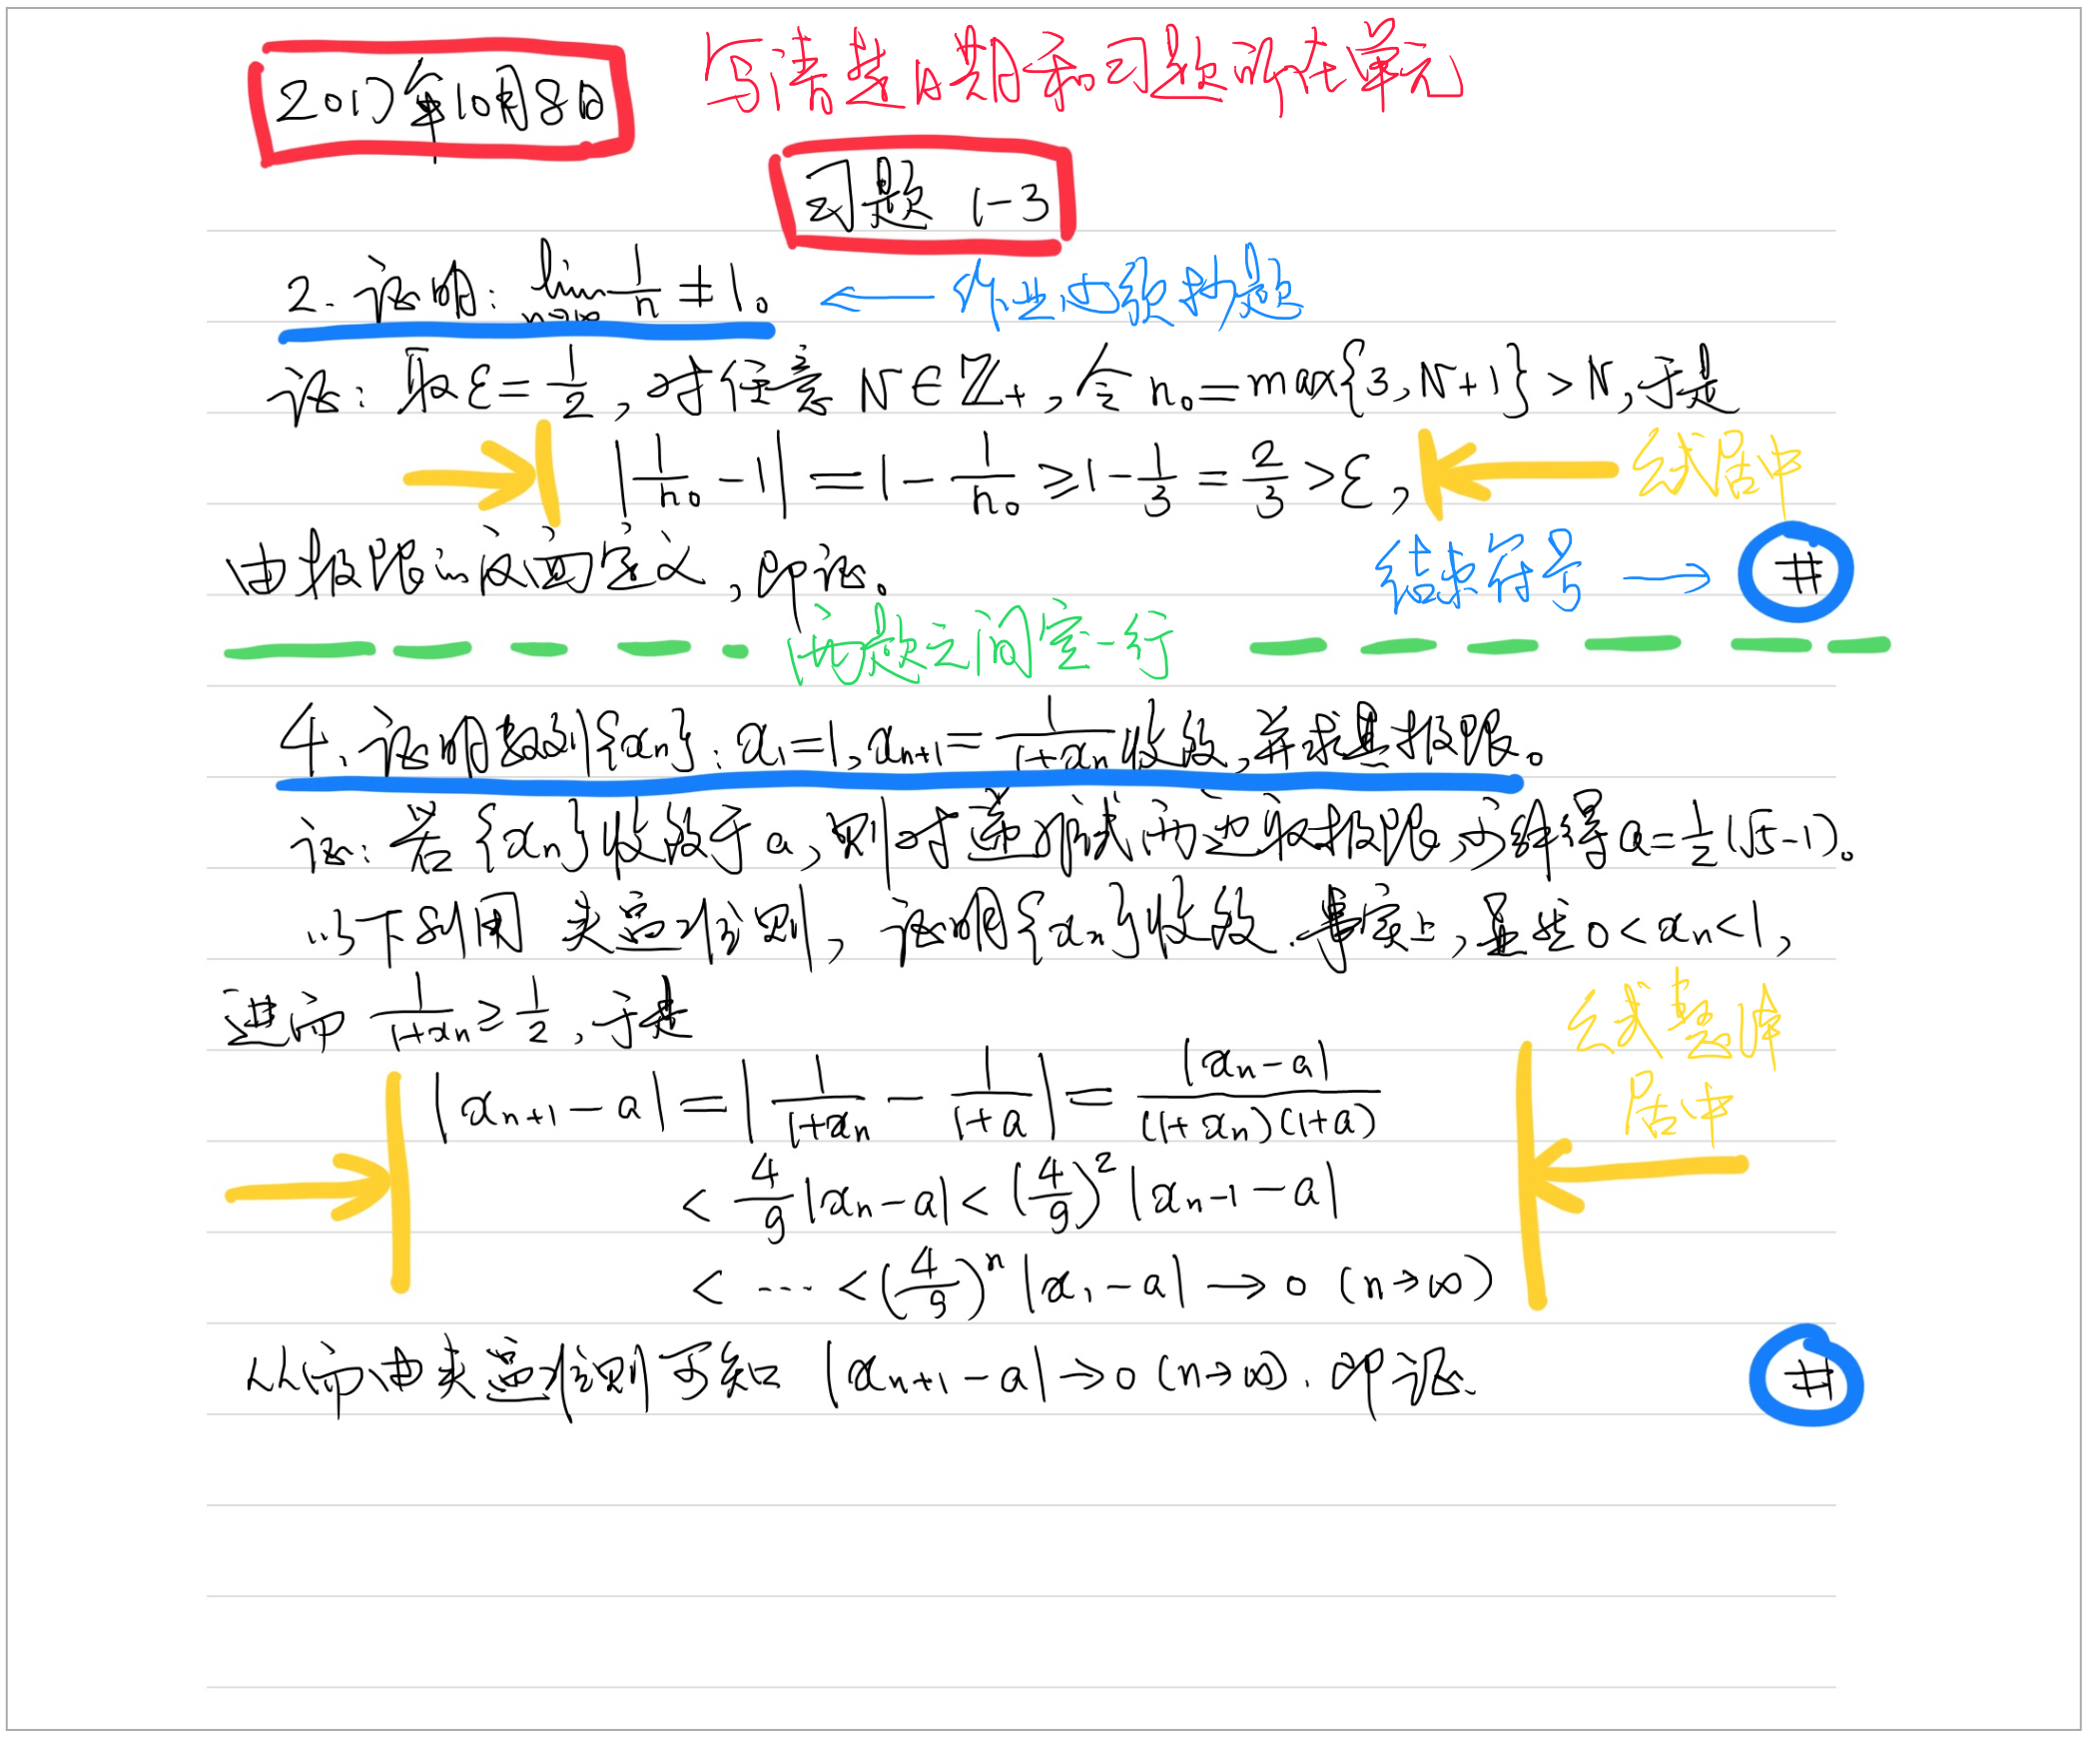
\includegraphics[width=0.95\textwidth]{./images/00/hw-sample.jpg}
  	
  	作业书写参考样式({\it 以黑色字体为准,彩色部分为格式说明})
  \end{center}
  \begin{itemize}
    \item 作业书写的规范
    \begin{enumerate}
      \item 写清楚作业日期(对应讲课的日期)和习题所在单元;
      \item 作业必须抄题,写清楚题号
	  \item 解题过程以“证:”或“解:”开始,以$\#$号结束;
	  \item 公式整体居中书写;
	  \item 无论大题小题,两题之间空一行;
	  \item 不允许使用铅笔、红笔书写作业,可以用铅笔画图;
	  \item 作业本不许分栏使用;
	  \item 文字、符号书写清晰规范,尽量少涂改。
    \end{enumerate}    
    \item no copy ??!
    \item 及时订正错误,补上缺漏
  \end{itemize}
	\item {\bf 答疑}
	  \begin{itemize}
	    \item 每周一次面对面答疑,1-2小时
	    \item 提问题的能力不完全是天生的,脸皮要厚一点
	    \item 综合利用各种手段(微信、网站、邮件、\ldots)
	  \end{itemize}
% 	  \item {\bf 从善如流}
\end{itemize}

\section{关于考试}

以下是2017-2018学年开始实施的“{\it 新政}”:

考试分为{\it 形成性考试}和{\it 终结性考试}两个部分,两部分成绩按照$40\%$和$60\%$的比例综合
得到最终的课程期末成绩。

每学期末设一次终结性考试,采用闭卷笔试形式。{\color{red}\bf 终结性考试不及格,
则课程成绩不合格!}

每学期的形成性考试分为四个部分,一是{\it 平时作业和表现}成绩,占$10\%$,剩下的为三次
{\it 单元测试}成绩,各占$10\%$。

单元测验的形式为笔试或网络测试,具体待定。

\bigskip

\begin{ext}
	{\centering\bf 课后作业}
	
	{\b\it 说明:作业必须写明题目所在章节、页码、题号;如非特别说明,
	所有题目必须抄题;两道题之间空一行;未作或作错的题目讲评后务必及时订正。}
	
	\begin{itemize}
	  \item 注册加入课程网站:https://www.trustie.net/courses/1259,邀请码:YRKWF
	  \item 注册中学大学MOOC账号:http://www.icourses.cn/imooc/,将用户名告知课代表
	  统一登记
	  
	  {\b\it 下面的题目请写在活页纸上,不用抄题:}
	  \item 写一篇短文,内容及要求如下
	  \begin{enumerate}[(1)]
	    \item 你的个人介绍,请务必包含如下信息:姓名、性别、年龄、籍贯、中学母校的名字、
	    你的高考总成绩(以及当地的满分)、你的高考数学成绩(以及当地的满分);
	    \item 你的兴趣爱好、特长,或者说,你觉得自己有什么与众不同之处;
	    \item 你学习数学的体会,例如:喜欢,不喜欢?喜欢什么样的数学,不喜欢什么样的数学?
	    有什么好的学习方法?有什么自己觉得成功的经验,或者有趣的经历(最好与数学有关)?
	    \item 你期待中的大学课堂是怎样的?怎么的教与学会对你更有帮助?对老师有什么期待、要求,
	    或者建议?
	    \item 请至少推荐一本(部、套)你喜欢的书、电影或者其他任何可以通过公共渠道获取到的资料
	    (例如:网站、软件、APP、\ldots),说说推荐的理由;
	    \item 其他任何你认为值得(可以)与我交流的东西,比如你想问我什么问题;
	    \item 除第一条必须包含外,其余内容可自由取舍。
	    \item 篇幅:不少于半页,不多于两页(一张纸的正反面)。
	  \end{enumerate}
% 	  {\b\it 以下的题目写在作业本上,作业本第一页背面上贴上一张个人的照片,标注专业和籍贯}
% 	  \item 习题1-2:5(3,4),7,8
% 	  \item 习题1-3:5(3),6(2),7,8
% 	  \item 习题1-4:7,8
% 	  \item 习题1-5:3
% 	  \item 习题1-6:4(2,3,5)
% 	  \item 习题1-7:4(2),5(3,4)
% 	  \item 习题1-8:4
% 	  \item 习题1-9:2,3(3,5,6),4
% 	  \item 习题1-10:1,5,7
% 	  \item 总习题一:14
	\end{itemize}
\end{ext}

\newpage

\begin{shaded}
	{\bf\Large Cornell Note-Taking System}\hfill{\it 康奈尔笔记法(5R笔记法)}
	
	\bigskip
	
	这一方法适用于一切依赖讲授或自学的学习过程,特别是对于听课笔记,5R笔记法堪称首选。
	该方法的重点是记与学、思考与运用的结合,以及将笔记的记录与完善作为学习的过程载体。
	最终完成的笔记类似于下图:
	
% 	\begin{figure}[htbp]
% 		\centering
% 		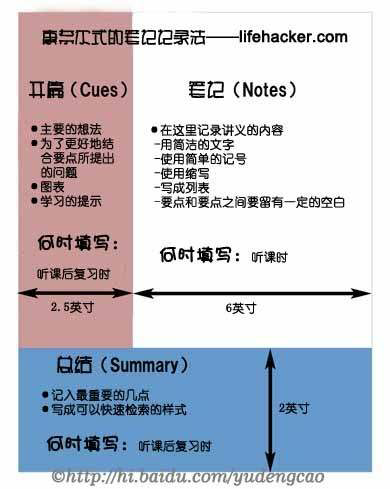
\includegraphics[width=0.4\textwidth]{./images/00/Cornell-NTS/NTS-CH.jpg}\quad
%  		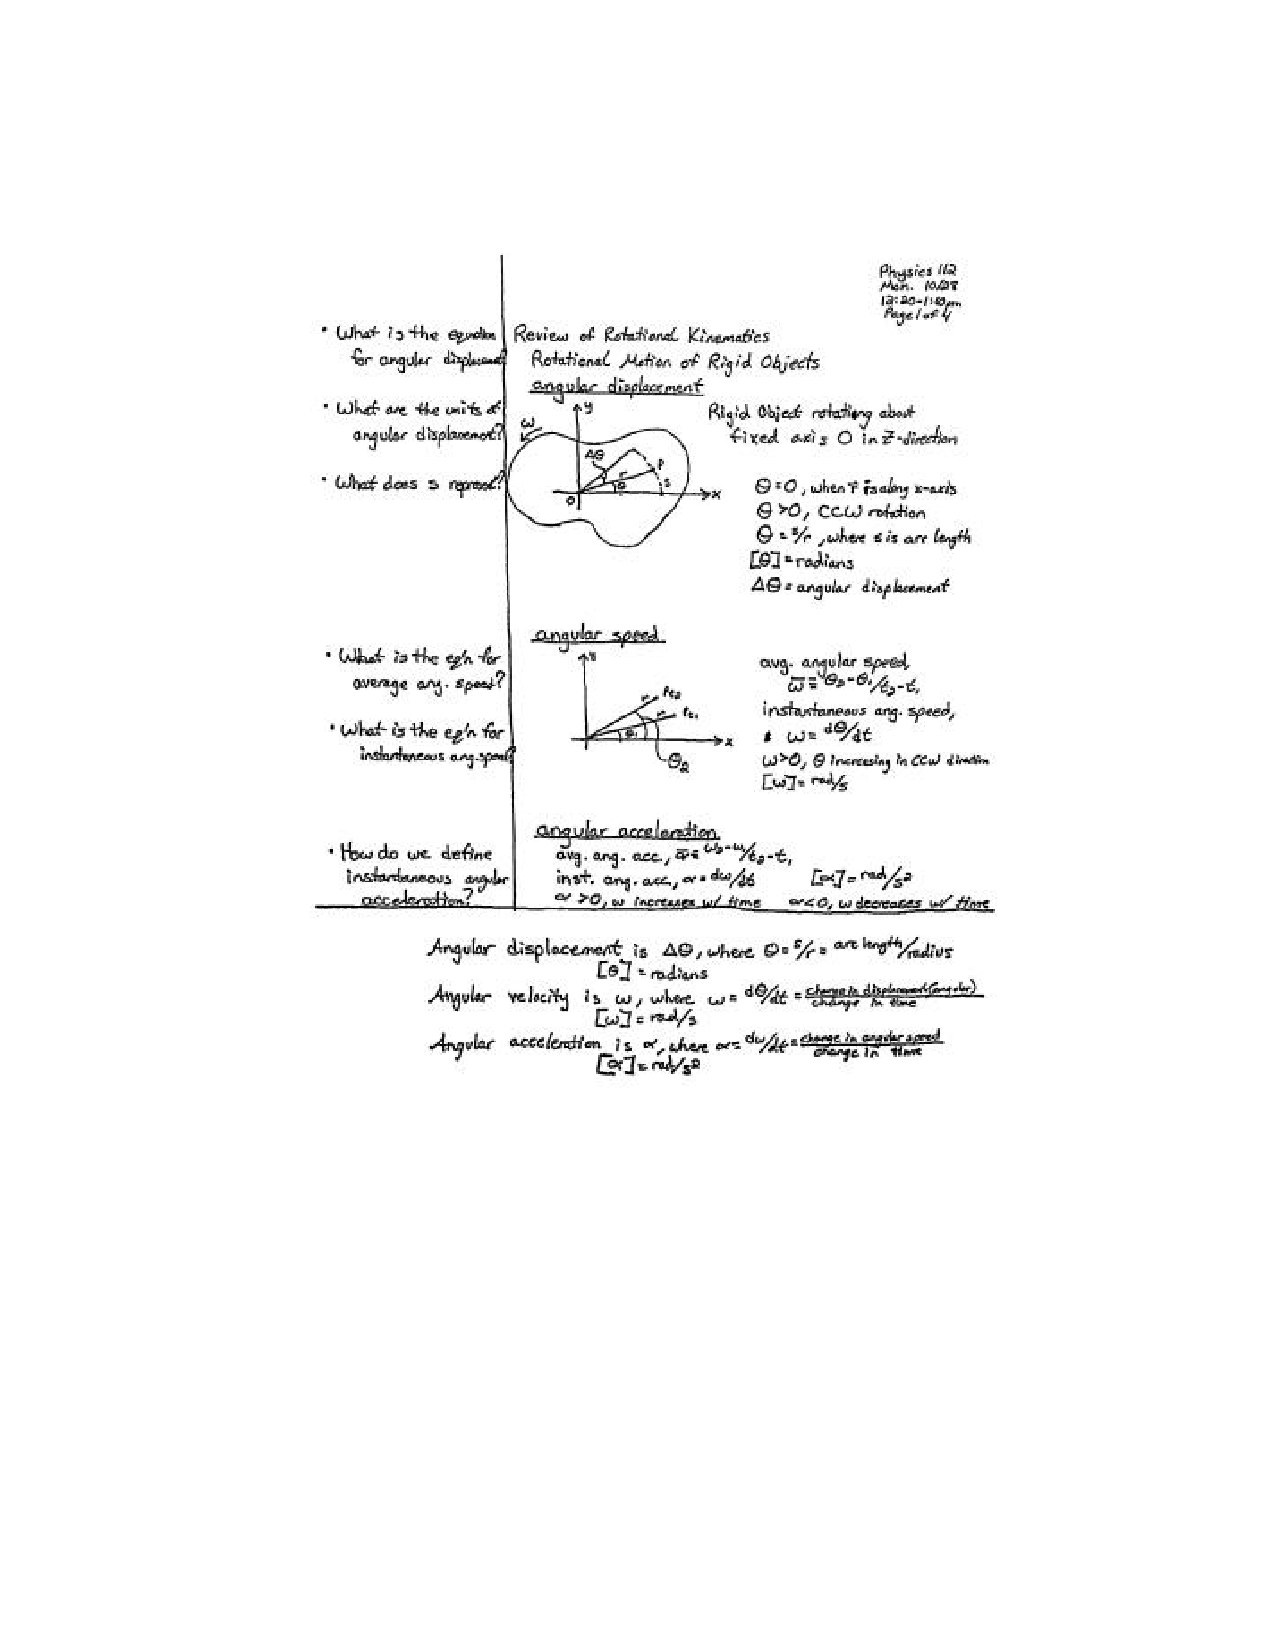
\includegraphics[height=8cm]{./images/00/Cornell-NTS/exCNTS.pdf}
% 	\end{figure}
	
	\begin{center}
		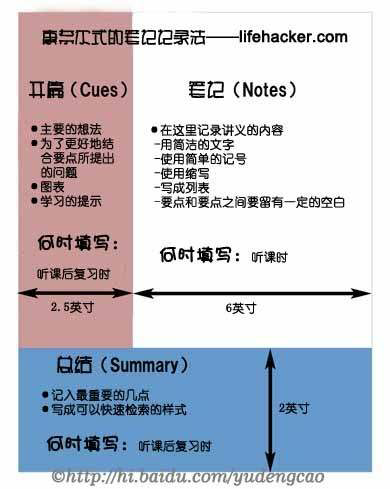
\includegraphics[height=8cm]{./images/00/Cornell-NTS/NTS-CH.jpg}\quad
		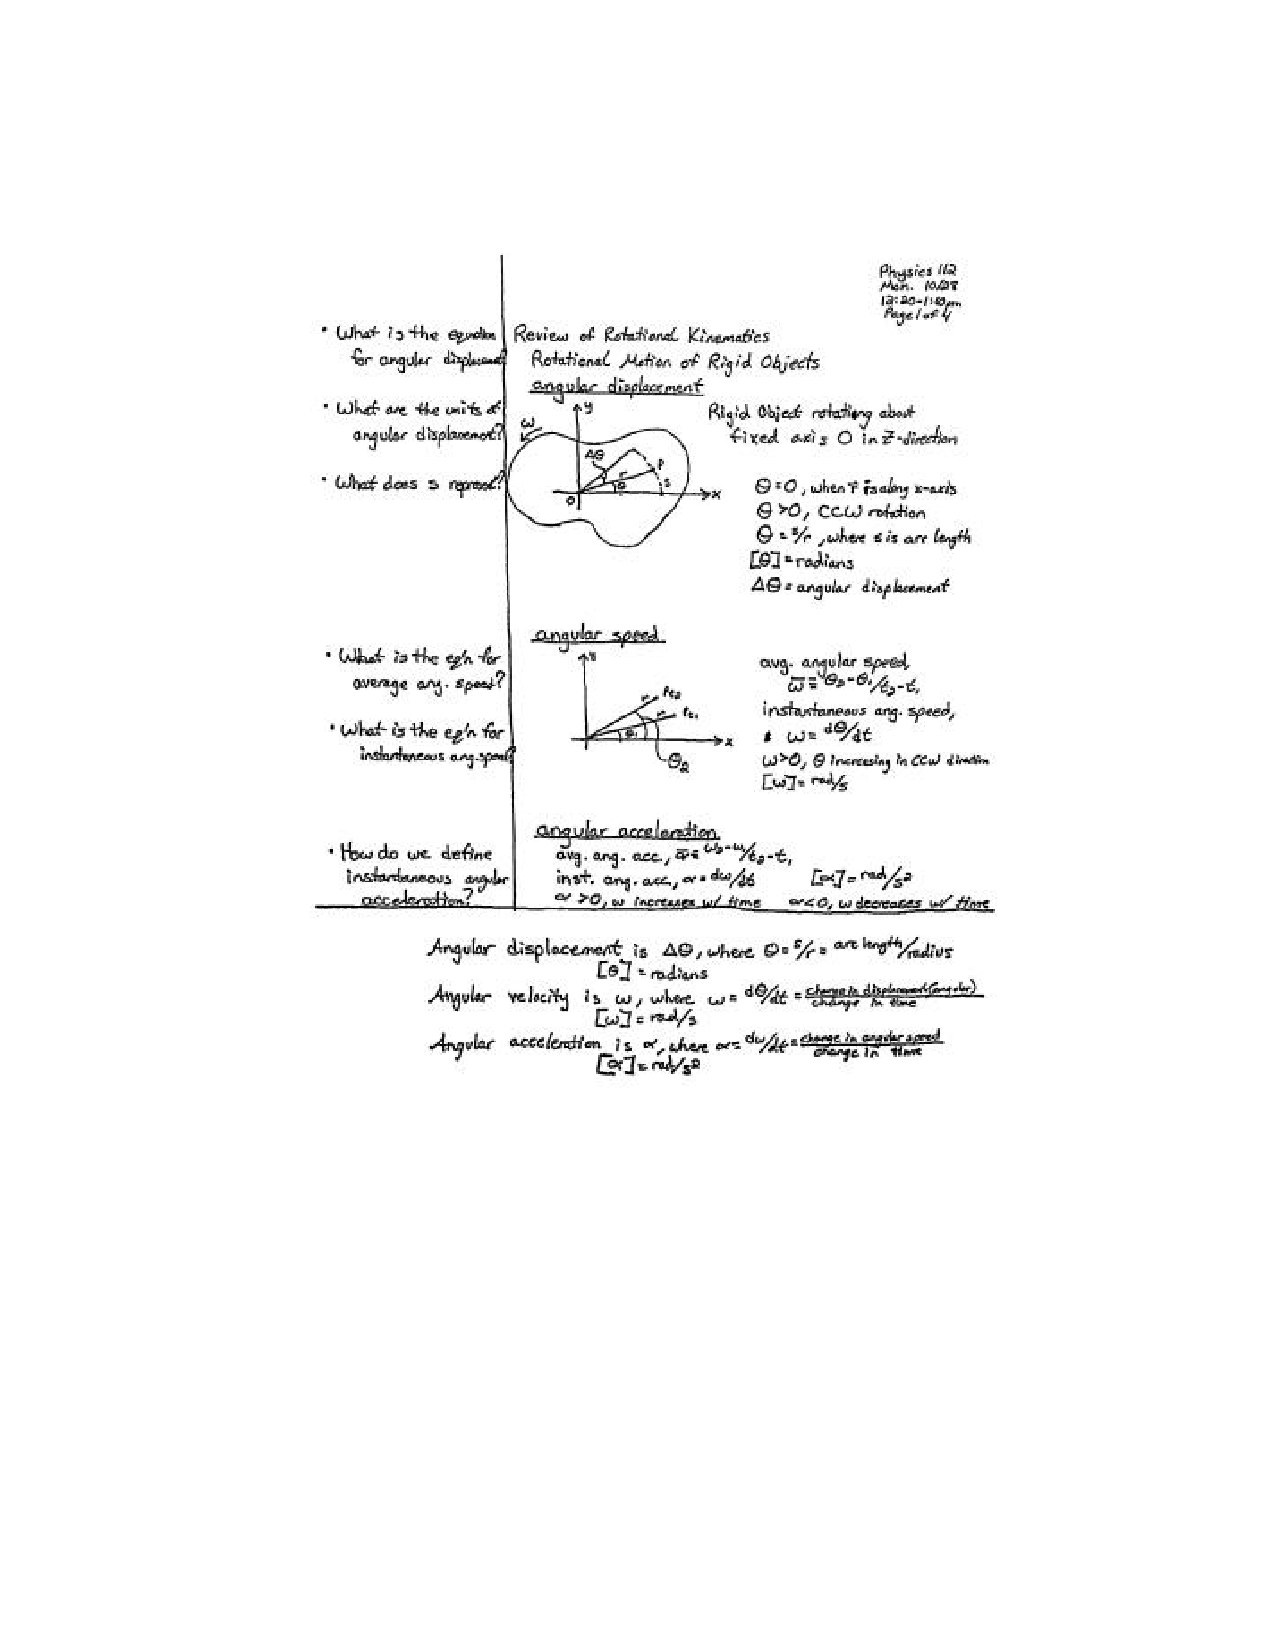
\includegraphics[height=8cm]{./images/00/Cornell-NTS/exCNTS.pdf}
	\end{center}
	
	笔记的行程过程可以分为所谓的{\bf 5R}:
	
	\begin{enumerate}[Step1]
	  \setlength{\itemindent}{1cm}
	  \item {\it 记录(Record):}在听讲或阅读过程中,
	  在主栏(将笔记本的一页分为左大右小两部分,
	  左侧为主栏,右侧为副栏)内尽量多记有意义的论据、概念等讲课内容。
	  \item {\it 简化(Reduce):}下课以后,尽可能及早将这些论据、概念简明扼要地概括(简化)
	  在回忆栏,即副栏。
	  \item {\it 背诵(Recite):}把主栏遮住,只用回忆栏中的摘记提示,
	  尽量完满地叙述课堂上讲过的内容。
	  \item {\it 思考(Reflect):}将自己的听课随感、意见、经验体会之类的内容,
	  与讲课内容区分开,写在卡片或笔记本的某一单独部分,加上标题和索引,
	  编制成提纲、摘要,分成类目。并随时归档。
	  \item {\it 复习(Review):}每周花十分钟左右时间,快速复习笔记,主要是先看回忆栏,
	  适当看主栏。
	\end{enumerate}
	
	在课本、参考书原文的旁边加上各种符号(如直线、双线、黑点、圆圈、
	曲线、箭头、红线、蓝线、三角、方框、着重号、惊叹号、问号等等),便于找出重点,
	加深印象,或提出质疑。什么符号代表什么意思,自己掌握即可,但最好形成一套比较
	稳定的符号系统。这种方法特别适合于自学笔记和预习笔记。
	
	操作时注意以下一些准则:
	{\it 读完后再做记号,要非常善于选择,用自己的话进行注记,形式和过程力求简洁,迅速,整齐}
	
	笔记的加工:{\it 忆$\to$补$\to$改$\to$编$\to$分$\to$舍$\to$记}	
\end{shaded}
